\section{Technical Design}\label{sec:technical-design}
%\lipsum[2-8]
At the end of Section~\ref{sec:op-params} it was shown that using the raw position readings coming from the sensor was not feasible in cases where NLOS is present.
Furthermore, the overall goal is for the position of an indoor UAV to be recovered with a fair amount of accuracy since this forms the basis of any autonomous behaviour and navigation.
As such it is desirable to use readings from multiple sensors but at the same time reducing the overall physical footprint of the final system to keep it lightweight.
With that in mind, it was proposed to directly integrate the POZYX sensor system with a motherboard unit that is capable of doing sensor fusion, UAV control, and communicating with external systems.
In recent years FCU's have become versatile and robust and these requirements are easily met so in this section the technical parameters of the research will be discussed.

\subsection{Flight Controller Unit}\label{subsec:flight-controller-unit}
In order to prevent consuming too much time on determining a suitable flight system the Open-Source Hardware (OSH) community was consulted in order to find a suitable FCU for the research.
Survey work done by ~\citet{ebeid2018survey} presents a qualitative analysis of several commercial hardware solutions.
Table~\ref{tb:comparison} shows some of the major hardware considerations.
All of the units have the standard UART, PWM and I2C interfaces in addition to other onboard sensors and interfaces.
At the time of writing the Pixhawk series of FCU's are the most common and oldest systems.
They have all the standard interfaces as well as several sensors allowing making them a keen choice for developers and researchers in a plug and play platform.
Many in the series share the same interfaces with some of the smaller boards excluding some of the less popular interfaces.
As such, to allow for flexibility in the technical design the Pixhawk line was chosen for this research.
After deliberation and consulting the objectives and scope of this research it was determined that a basic Pixhawk would be satiable.
Figure~\ref{fig:pix} shows the board chosen, it was shipped quickly and it contains everything necessary to meet the objectives of the project allowing for quick prototyping and proof of concepts.

\begin{table}[h!]
    \centering
    \begin{tabular}{|c | c | c | c | c|}
        \hline
        Platform & MCU & Sensors & Licenses & Interfaces\\
        \hline
        Pixhawk & STM32F427 & b, m & BSD & c, s, a, pp, sb, ds\\

        Pixhawk2 & STM32F427 & b, m & CC-BYSA-3.0 & c, s, a, pp, sb, ds\\

        PixRacer & STM32F427 & b' m & CC-BY 4.0 & c, pp, sb, ds \\

        Pixhawk 3 Pro & STM32F427 & b' m & CC-BY 4.0 & c, s, pp, sb, ds \\

        PX4 FMUv5 and v6 & STM32F427 & b' m & CC-BY 4.0 & c, s, a, pp, sb, ds \\

        CC3D & STM32F103 & None & GPLv3 & pp, ds, sb\\

        APM 2.8 & ATmega2560 & b & GPLv3 & pp, a\\

        Erle-Brain 3 & Raspberry Pi & b, m & CC BY-NC-SA &  a\\

        PXFmini & Raspberry Pi & b, m & CC BY-NC-SA & a\\
        \hline
    \end{tabular}
    \caption{Comparisons of various FCU's that are commercially available.
    Source: ~\citet{ebeid2018survey} Page: 2.}
    \label{tb:comparison}

    Legend:\\
b: barometer, m: magnetometer, p: pitot tube sensor, c: CAN, s: SPI, a: ADC, pp:
PPM, sb: S.BUS, ds: DSM, da: DAC, x: XBEE, au: AUX, [d]: discontinued.
\end{table}

\begin{figure}[ht!]
    \centering
    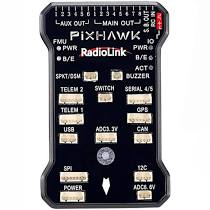
\includegraphics[scale=0.7]{mtd/pixhawk}
    \caption{Radiolink Pixhawk used for the project}
    \label{fig:pix}
\end{figure}

Furthermore, since the chosen board is OSH it has several options of firmware that can be used.
This made code and software developed on this system extendable to other boards given they are able to run the firmware.
\newpage

\subsection{Flight Firmware}\label{subsec:flight-firmware}
Now that a suitable FCU was chosen the next major step was determining a flight stack to run on the board.
The major firmware options for the Pixhawk are either Ardupilot or PX4 stack.
Both are well documented and have their advantages.
Both support a large array of vehicles but the major differences come from the licenses they are under.
Without delving into the technicalities of the licenses it is often summarised that PX4 is attractive to business owners who want to protect their property whilst Ardupilot pushes for changes to be put back into the main codebase.
Additionally, from a evaluation of each of the firmware, Ardupilot is slightly more documented due to its general public license and a bit more user friendly in terms of compilation and flashing firmware thanks to its pythonic based wrapper for compilation and uploading.
Since both firmware cover all the generic UAV types and there was no need for any niche systems Ardupilot was chosen as the primary codebase.
It is worth noting that there is a subsection of the Ardupilot codebase dedicated to Beacon based positioning systems which a previous Pozyx implementation is coded ~\citep{ardupilotarduino}.

\subsection{Communication Interface (I2C vs Serial)}\label{subsec:communication-interfacei2c-vs-serial}
As mentioned in Chapter~\ref{ch:literature-review} there is an implementation using a Pozyx system in a GPS denied scenario ~\cite{ardupilotarduino}.
This shows that it is possible to get the positioning data into the Ardupilot codebase and have it interact with the onboard sensor fusion systems.
A critique of this approach, however, is that it uses an additional Arduino Uno to pipe information from the Pozyx tag to the Pixhawk.
Given the availability of the standard interfaces onboard the Pixhawk and the scope and objectives of this research project, it is feasible that the Uno can be stubbed out of this experiment and data can be integrated directly onto the Pixhawk.
This means the physical integration of the system can be summarised into the following steps:
\begin{itemize}
    \item Choosing a suitable interface.
    \item Placing the code within a suitable section of the codebase.
    \item Utilise the parent class of the section of the Ardupilot to integrate the sensor.
    \item After testing the base functionality, integrate the new library within the background scheduler so it can run and feed measurements in the background to the copter main code.
\end{itemize}

Arduino and python libraries ~\citep{pozarduino} were originally designed by the Pozyx developers so it provided an algorithmic starting point for the functionality of the library being designed.
The Arduino library is based around the I2C protocol whilst the python module uses the serial interface.
As noted by the developers the python module is a port of the Arduino library and there are no plans to maintain the code and address bug fixes, as such the Arduino library was studied to build the new AP\_Bacon extension.
Furthermore, the I2C interface was designed onboard an embedded system so much of the flow can be ported effectively to the Pixhawk.
Lastly, the previous implementation uses the UART/serial interface so that avenue has already been explored, in the interest of quick prototyping the I2C interface was chosen.
A positive note is that the existence of the prebuilt system allows data and experiments to be collected in lieu of the development of this library since the information being provided is the same data generated by the Pozyx tag.
The design of this library proves that the sensor data can be integrated directly whilst the pre-built systems, which are stable, can be used for data collection and experiments.
%
%\begin{figure}[h!]
%    \centering
%    \includegraphics[scale=0.5]{}

%\end{figure}

\begin{figure}[ht!]
    \centering
    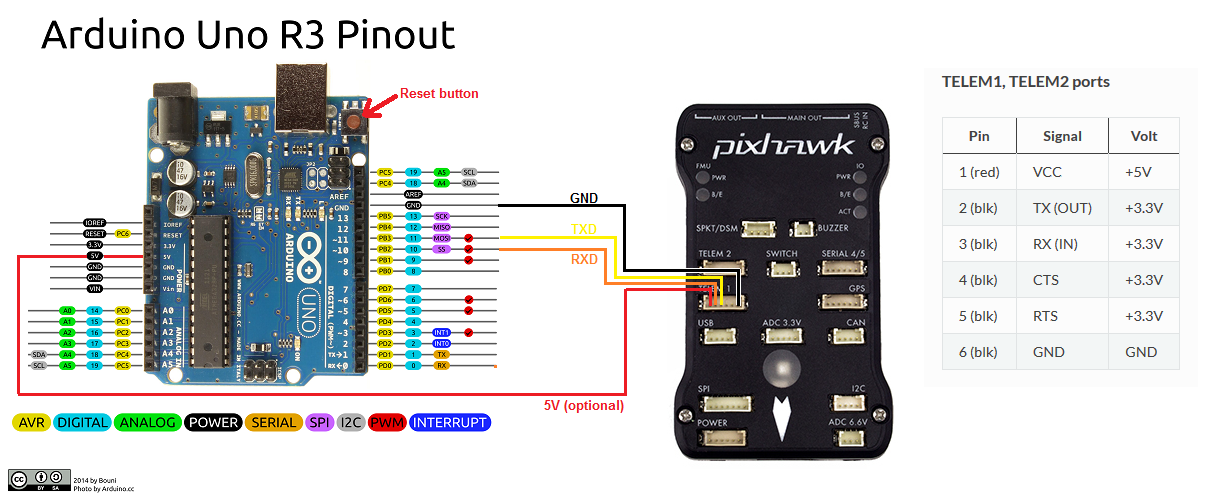
\includegraphics[width=\textwidth]{mtd/pozyx_uno}
    \caption{Non-GPS loiter solution provided by Ardupilot.
    Source:\url{https://ardupilot.org/copter/docs/common-pozyx.html}}
    %    \label{fig:pix}
\end{figure}

\begin{figure}[ht!]
    \centering
    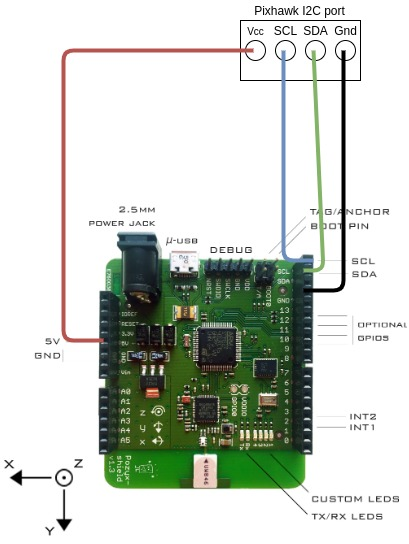
\includegraphics[scale=0.6]{mtd/i2c_ifc}
    \caption{Proposed wiring of the I2C interface being developed}
\end{figure}

\begin{figure}[ht!]
    \centering
    \includegraphics[width=0.85\textwidth]{mtd/wip}
    \caption{System being unit tested in the environment.}
\end{figure}
\newpage
\subsection{Sensor Fusion: Pozyx Readings and EKF on Ardupilot}\label{subsec:sensor-fusion}
As mentioned in Chapter~\ref{ch:literature-review} sensor fusion forms the basis of estimating states of the system when there are multiple measurements of that state present.
The de facto one used in navigation and localisation happens to be the Extended Kalman Filter (EKF).
The Ardupilot codebase implements an EKF to estimate 24 states.
The state being affected by the implementation will be the position estimates given in North, East, Down (NED) frame.
The NED reference frame is similar to the standard left-handed notation used in several standard robotic systems with the major difference being the Down axis which is opposite in direction to the standard Z axis in robotic systems.
The developers of the Pozyx system, ~\cite{pozyx2018pozyx}, designed the firmware of the tag in such a way that obtaining information or triggering any functions can be done with sequential reading and writing operations to various registers on the tag.
~\citet{devregs} lists all the functionality of the tag via the registers.
From the registers, it is possible to obtain both the distances of the tag to each anchor as well as the position of the tag within the workspace.
It was confirmed by developers that the positioning algorithms operate in two modes.
\begin{enumerate}
    \item A pure triangulation using the TOF readings from each anchor.
    \item A tracking mode which combines IMU and TOF readings in a Kalman Filter to improve accuracy.
\end{enumerate}
For the purpose of this research, the position readings were used since these can be directly integrated into the Ardupilot codebase immediately.
Furthermore, the tag was configured to be used in the tracking mode to improve the accuracy of the measurements.
Lastly, from Section~\ref{sec:op-params} and notes from the Pozyx team and ~\citet{evaluwb} four anchors may not provide sufficient data for a full 3D position so the system was hardcoded to operate in a 2.5 dimension which means the height (z reading) was fixed on a surface so the tag calculated and provided (x,y, z reading) positioning when requested.
The final step was to have this implemented on the Pixhawk with the Ardupilot firmware within the Beacon subsystem of the code.
This meant that the following steps had to be implemented.
\begin{itemize}
    \item Initialise the I2C bus on the Pixhawk and configure the tag.
    \item On an 'update()' function call, set the vehicle position based on the tag reading and set the distance between each anchor and the tag.
    \item A 'healthy()' function call, should return true if the Pixhawk was able to retrieve viable data from the tag.
\end{itemize}

Appendix~\ref{app:app02} shows the core code designed to do this but the overall integration with the Ardupilot codebase can be seen by the pseudo-code below.
\begin{algorithm}
    Main vehicle code
        loop()
        {
            beacon_reading = beacon->get_vehicle_position()
            EKF_update()
            {
                ...
                fusebcnreading()
                ...
            }
            .
            .
            .
    Background Scheduler
        loop()
        {
            ...
            beacon->update()
            ...
        }

        }
\end{algorithm}

Appendix~\ref{subsec:ap_pozyx_test.cpp} also shows a test to ensure the standard interface and data encapsulation is exactly what is needed and provided by the other beacon measurement systems in the Ardupilot codebase.
Although it was verified that the code was integrated and the measurements were being captured by the main vehicle code and EKF measurement function operating indoors prevented the internal compass/magnetometer from working properly.
When the compass is disabled the 'yawAlignComplete' check, which is required by the EKF to see if beacon measurements are viable to use, is set whilst the UAV is in flight.
Due to only having access to an FCU at the time, the onboard EKF estimates could not be obtained and sent via MAVLink without a refactor to the core code which is outside the scope of this research project.
However, to rectify this a simple two state EKF's were implemented in python and on a mobile robot to determine if viable position estimates could be generated that can be used in a UAV or robotic system.

\subsection*{EKF Design}
As discussed in Section~\ref{sec:sensor_fusion} and the preceding section an EKF was implemented to improve the position estimates from the Pozyx sensor.
The major driving force for using an EKF over other filters and estimators was to mimic the Ardupilot setup as closely as possible as to promote future work and testing of the UAV whilst in flight.
Once again the tag will be operated in 2.5 dimensions in tracking mode to determine if the system can withstand NLOS when dynamic obstacles are introduced into the environment.
Similar to the setup in Section~\ref{sec:op-params} the tag was allowed to operate and record in various scenarios while static and moving.
It should be noted that since we are operating in 2.5 dimensions a two state filter will be implemented.
Furthermore, since the tag outputs direct measurements of the state the matrices are simplified and easy to implement.

System equations:
\begin{equation*}
    \begin{split}
        f(\hat{x},\hat{u},t) = \left[ \begin{array}{cc}
                              x & 0\\
                              0 & y
        \end{array} \right]\\
        z(\hat{x}) = \left[ \begin{array}{cc}
                              x & 0\\
                              0 & y
        \end{array} \right]\\
    \end{split}
\end{equation*}


Linearised state transition model:
\[
    F =
    \left[ \begin{array}{cc}
    1 & 0\\
    0 & 1
    \end{array}
    \right]
\]

Linearised observation model:
\[
    H =
    \left[ \begin{array}{cc}
    1 & 0\\
    0 & 1
    \end{array}
    \right]
\]

An added benefit of using the Pozyx sensor is that it is possible to obtain the measurement uncertainty for each measurement which allows it to be incorporated in the calculation of the Kalman Gain at each time step.

\[
    R =
%
        \left[
            \begin{array}{cc}
                Var(x)(t) & Cov(x,y)(t)\\
                Cov(x,y)(t) & Var(y)(t)
            \end{array}
        \right]
\]

Another adjustment from the standard EKF is that outlier measurements were not used.
Outliers arose due to sudden jerks in motion causing the measurements coming out of the tag to be erratic and vary wildly in certain time steps.

The above EKF design represents a pure pythonic approach using only the readings from the sensor.
Given that it only has once set of observations it can be considered a simple filter rather than a state estimator.
To emulate the process that should run on the Pixhawk is is desirable to actually incorporate another stream of measurements that would improve the position estimates.
To this end, an EKF was applied on a wheeled mobile robot running dead reckoning localisation.
To easily fuse the dead reckoning readings, the robot sensors were simplified to outputting the $(x,y)$ position based on left and right wheel encoder readings.
Additionally, the board is Arduino based so integration with the Pozyx system is straightforward.
Figure~\ref{fig:poz_romi} shows how this system was connected and used.

This following system of equations shows the EKF on the wheeled mobile robot:

\begin{equation*}
    \begin{split}
        f(\hat{x},\hat{u},t) = \left[ \begin{array}{cc}
                              x & 0\\
                              0 & y
        \end{array} \right]\\
        z(\hat{x}) = \left[ \begin{array}{cc}
                              x_{tag} & 0\\
                              x_{encoders} & 0\\
                                0 & y_{tag}\\
                                0 & y_{encoders}
        \end{array} \right]\\
    \end{split}
\end{equation*}


Linearised state transition model:
\[
    F =
    \left[ \begin{array}{cc}
    1 & 0\\
    0 & 1
    \end{array}
    \right]
\]

Linearised observation model:
\[
    H =
    \left[ \begin{array}{cc}
    1 & 0\\
    1 & 0\\
    0 & 1\\
    0 & 1
    \end{array}
    \right]
\]

\[
    R =
%
        \left[
            \begin{array}{cccc}
                Var(x)_{tag} & 0 & 0 & 0\\
                0 & Var(x)_{encoders} & 0 & 0\\
                0 & 0 & Var(y)_{tag}& 0 \\
                0 & 0 & 0 & Var(y)_{encoders}
            \end{array}
        \right]
\]

\begin{figure}[ht!]
    \centering
    \includegraphics[width=0.85\textwidth]{mtd/romi_pozyx}
    \caption{Wheeled mobile robot equipped with the Pozyx Tag.}
    \label{fig:poz_romi}
\end{figure}

\section{Summary}
This section thoroughly discussed the methodology and design process used to achieve the objectives and scope of this research.
Although Ardupilo'st EKF could not be used due to several limitations and scoping of this project, the feasibility of an EKF, in general, was explored as a method of improving the
overall position estimates of the system which can then be extended for use in the future within an Ardupilot based FCU without the current limitations.
In the next chapter the results of the EKF will be presented under various scenarios to show the effectiveness and limitations of the Pozyx sensor in a household environment.
%\lipsum[2-6]